\chapter{Testes Automatizados de Interface Gráfica} \label{cap:tests}

\section{Definição do Projeto de Testes}
O projeto de testes da aplicação inicialmente previa apenas testes manuais, tanto a nível de código, quanto em relação à interface gráfica. Atualmente, a empresa Jungle Devs não tem uma estrutura formalizada para a implementação de testes automatizados em seus projetos de software. Testes manuais são realizados a cada final de \textit{sprint} por um time de garantia de qualidade, responsável por detectar problemas no sistema e por reportar os mesmos ao time de desenvolvimento.

O presente trabalho apresentou oportunidades para o início de um processo de estudo e implementação de testes automatizados dentro da empresa. Testes automatizados de interface gráfica podem ser realizados sem alterar a estrutura do software e o fluxo de trabalho da empresa. Esta característica se deve ao fato de se tratarem de testes do tipo caixa preta. Assim, optou-se por iniciar um projeto de testes experimental, a nível de interface gráfica, para avaliar possibilidades de adoção de testes automatizados dentro da empresa e a factibilidade do uso de ferramentas para este fim.

Os testes automatizados foram realizados com a interface do aplicativo já implementada. Como consequência, o projeto de testes teve início após o encerramento do ciclo de desenvolvimento da fase piloto do aplicativo. Assim, os testes foram tratados de forma isolada ao projeto do aplicativo, utilizando-se do mesmo apenas como cenário para um caso de estudo. Coube ao autor a responsabilidade completa pela condução do estudo dos testes.

A camada de testes automatizados de interface gráfica procura simular o comportamento do usuário final da aplicação. Assim, testes de aceitação são ideias para serem implementados neste nível. Dois casos de teste foram escolhidos para o estudo: fluxo de cadastro das academias e erros de cadastro do treinador. Ambos os casos pertencem a parte de cadastro do aplicativo. Estes foram escolhidos por se tratarem de cenários muito recorrentes em projetos de aplicativos, assim futuras implementações dentro da empresa podem se beneficiar deste trabalho.

\section{Ferramentas Escolhidas}
Os testes automatizados foram implementados com o auxílio de ferramentas específicas para este tipo de testes. Existem muitas opções de frameworks disponíveis, tanto proprietárias, quanto de código aberto. Neste projeto, optou-se pelo uso somente de ferramentas de código aberto, por serem de fácil acesso e terem bom suporte oferecido pela comunidade de software (desenvolvedores independentes e empresas).

Existem ferramentas com suporte específico para determinadas plataformas e outras que podem servir casos para múltiplas delas. O desenvolvimento do aplicativo Gyymi foi requisitado para duas plataformas: Android e iOS. Assim, um ferramenta que suportasse diferentes sistemas operacionais foi escolhida, o Appium \cite{appium}. E devido ao fato do aplicativo apresentado neste trabalho ser voltado ao sistema iOS, outra ferramenta específica para a plataforma em questão também foi selecionada, o EarlGrey \cite{earlgrey}.

Além do Appium e do EarlGrey, também foi considerado a utilização da suíte de testes integrada ao Xcode, denominada XCUITest \cite{xcuitest}. Porém nenhum dos casos de teste implementados utilizou o XCUITest, pelo fato do desenvolvimento com o EarlGrey ser julgado suficiente para contemplar o uso de ferramentas específicas de plataforma. A ferramenta Appium foi a mais utilizada por apresentar maior potencial de reuso, tendo os dois casos de teste sido implementados com a mesma. O EarlGrey foi utilizado apenas no primeiro cenário de testes.

\section{Pré-configurações e Setup das Ferramentas}

\subsection{Modificações no Projeto}
A estrutura do código fonte do projeto manteve-se inalterada, contudo algumas adaptações foram realizadas para permitir as implementações. Os testes de interface gráfica foram desenvolvidos de modo a reconhecer componentes através da identificação de acessibilidade. Estas identificações não haviam sido criadas na fase de desenvolvimento do piloto e, portanto, tiveram que ser adicionadas aos componentes da interface que foram utilizados nos casos de teste.

\subsection{Appium}
A utilização do Appium foi feita através da API disponível para a linguagem Python. A escolha da linguagem se deve ao fato do autor já estar familiarizado com sua sintaxe e, também, pela empresa utilizar a linguagem em outras stacks, como no back-end. O código em Python foi escrito com editor de text Visual Studio Code.

Além da API em python, o Appium necessita que um servidor web local seja instanciado. Este é responsável por intermediar as interações entre os comandos enviados da API e o dispositivo móvel que contém o aplicativo. Para que este servidor seja criado, existem duas alternativas: através da CLI do Appium (Figura \ref{fig:appium-cli}) ou pela GUI do Appium (\ref{fig:appium-desktop}). As duas opções foram testadas. A CLI é de fácil utilização, contendo apenas um comando principal. A GUI oferece opções de configurações mais acessíveis, além de outras funcionalidades, como a inspeção (Figura \ref{fig:appium-desktop-inspector}) da execução do aplicativo (permite a visualização da hierarquia dos componentes da interface).

\begin{figure}[H]
    \centering
    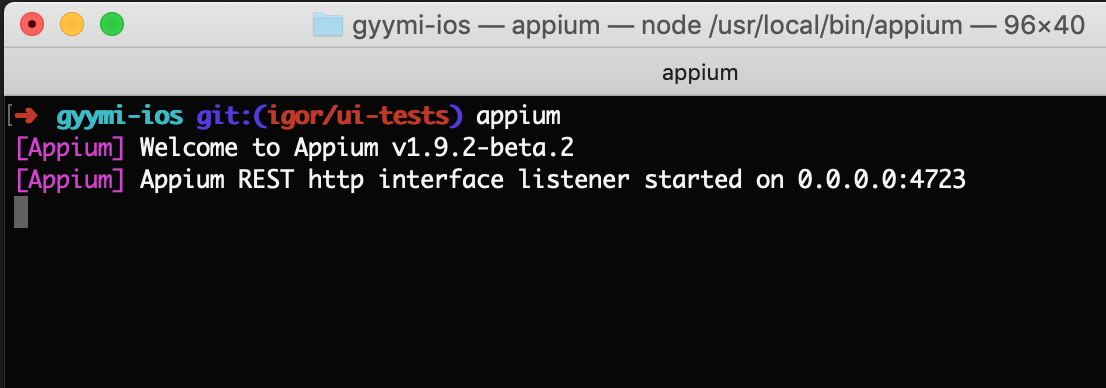
\includegraphics[width=0.8\textwidth]{pfc/figuras/appium-cli.png}
    \caption{CLI do Appium}
    \label{fig:appium-cli}
\end{figure}

\begin{figure}[H]
    \centering
    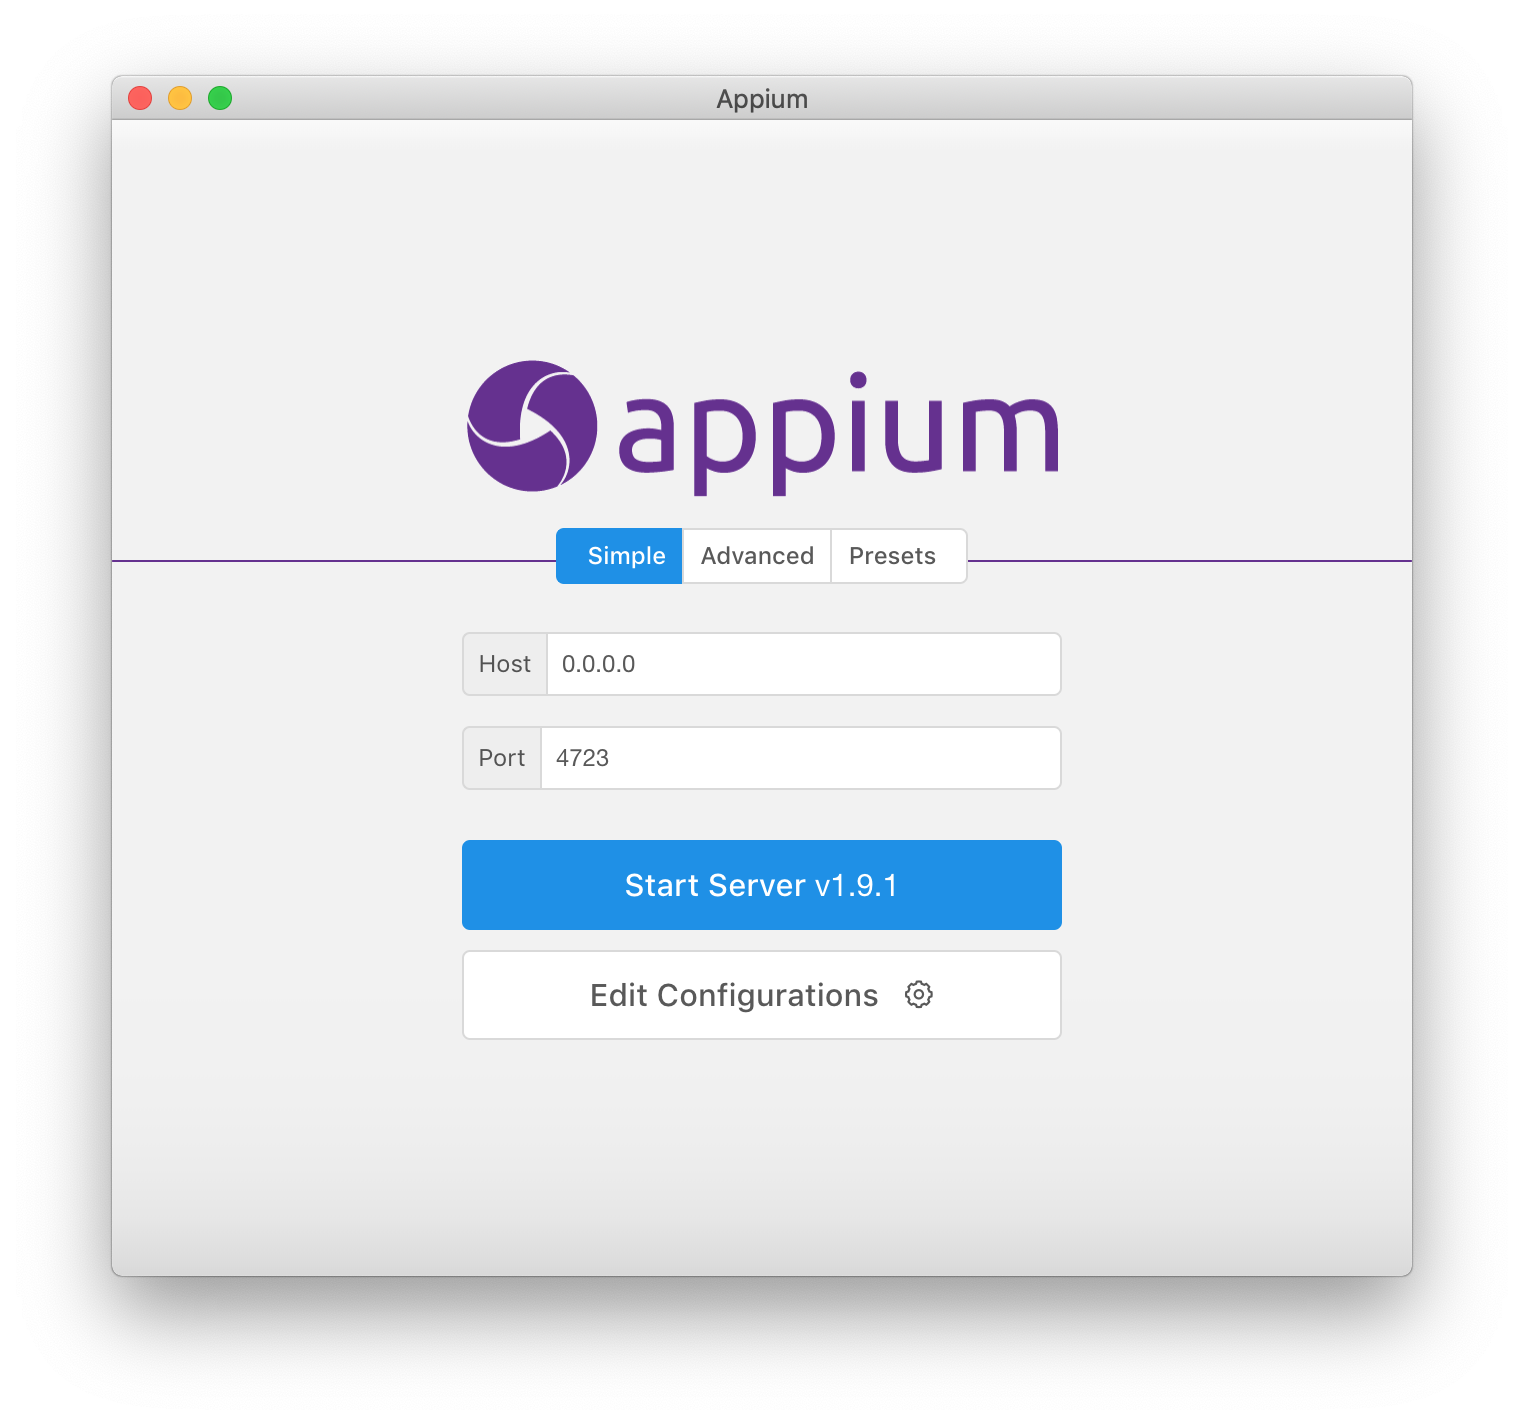
\includegraphics[width=0.8\textwidth]{pfc/figuras/appium-desktop.png}
    \caption{GUI do Appium}
    \label{fig:appium-desktop}
\end{figure}

\begin{figure}[H]
    \centering
    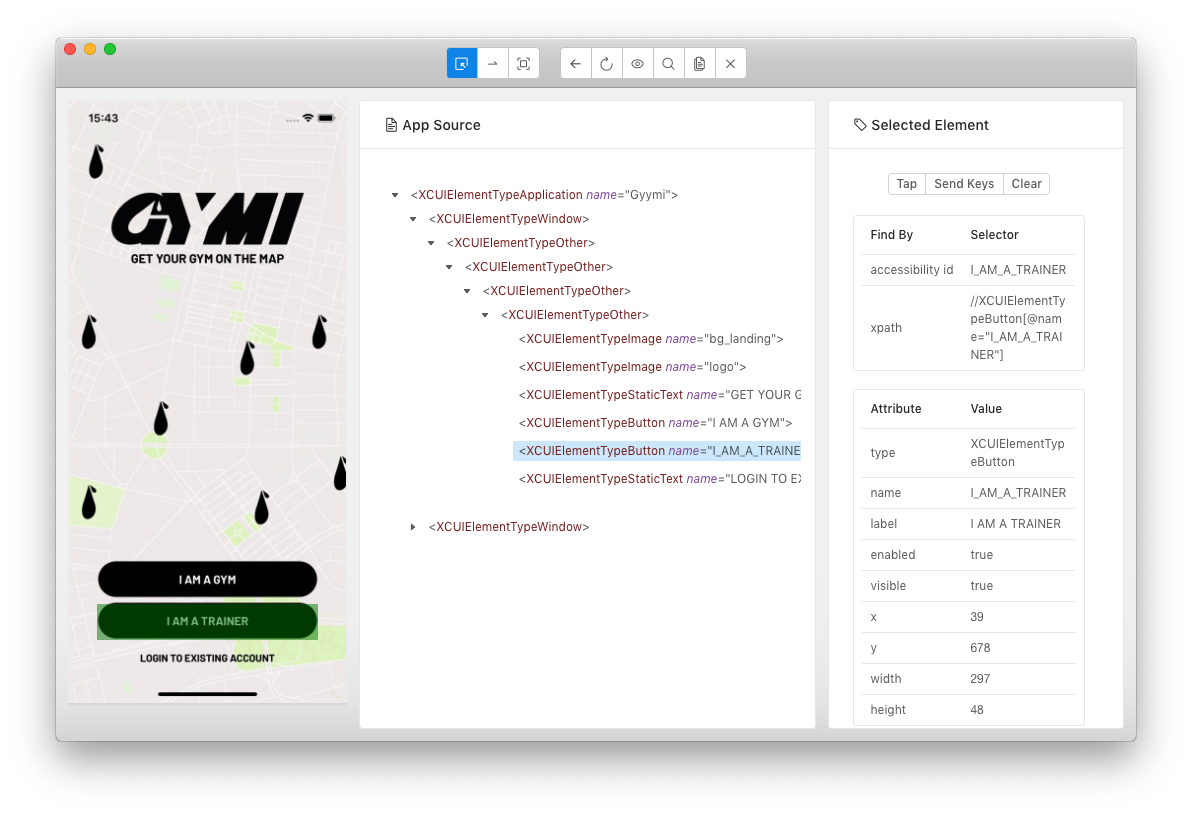
\includegraphics[width=0.8\textwidth]{pfc/figuras/appium-desktop-inspector.png}
    \caption{Ferramenta de inspeção do Appium}
    \label{fig:appium-desktop-inspector}
\end{figure}

\subsection{EarlGrey}
A configuração do EarlGrey requer menos passos, já que sua utilização é feita pelo Xcode. Primeiramente, um novo objeto de projeto (\textit{target} em inglês) dentro do Xcode foi criado para isolar o código de testes e o referente à aplicação. Assim, a compilação do código dos testes e da aplicação dá-se de forma separada, bem como a configuração de dependências para os dois casos. Por último, o EarlGrey é adicionado como dependência do código dos testes automatizados.

\section{Casos de Teste}

\subsection{Estratégia de Implementação}
A implementação dos testes seguiu o paradigma de programação orientado a objetos. A escolha da abordagem foi feita pelo fato do código do aplicativo também utilizar o paradigma como estrutura. A Figura \ref{fig:class-diagram-tests} apresenta o diagrama de classes para os casos de teste. Uma classe base foi criada para implementar os métodos comuns aos casos de teste, como chamadas para iniciar e encerrar gravações de vídeo, tirar fotos da tela e preencher campos de texto. Além disso, a classe base contém uma propriedade que referencia um objeto de geração de conteúdo (implementado por bibliotecas de terceiros), o qual simula a entrada de dados de um usuário real. Em seguida, uma classe foi criada para cada cenário de teste, contendo os métodos específicos para cada caso.

O código segue uma abordagem declarativa, isto é, são criadas camadas de abstrações através de funções que representam o que é realizado no teste. A estratégia tem o objetivo de possibilitar o reuso de código, aumentar a legibilidade e permitir que pessoas que não tem contato com as linguagens e ferramentas compreendam o que o código de teste realiza.

\begin{figure}[H]
    \centering
    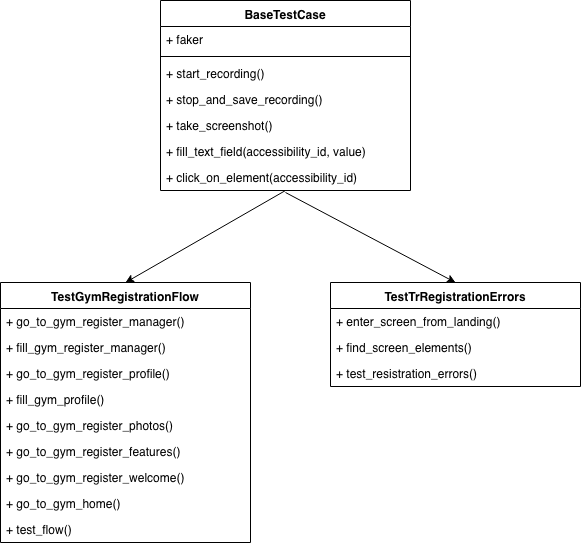
\includegraphics[width=0.8\textwidth]{pfc/figuras/class-diagram-tests.png}
    \caption{Diagrama de classes para os casos de teste}
    \label{fig:class-diagram-tests}
\end{figure}

\subsection{Fluxo de Cadastro das Academias}
Este primeiro caso tem como objetivo testar o fluxo de cadastro de academias no aplicativo. A sequência tem início na tela de entrada do aplicativo (Figura \ref{fig:landing}) e encerra-se ao final do cadastro (Figura \ref{fig:gym-welcome}). O teste tem sucesso se todas as etapas do cadastro são concluídas, ou seja, da perspectiva da interface gráfica, todas as telas de cadastro devem ser visualizadas. Garantir que este fluxo funcione da maneira esperada é de fundamental importância, uma vez que as principais interações no aplicativo ocorrem em torno da entidade da academia.

A implementação deste cenário de teste foi realizada no Appium e no EarlGrey. A Figura \ref{fig:test-flow} ilustra o trecho de código em que o método principal do caso de teste é chamado em ambas as ferramentas. Nota-se uma grande semelhança nos dois códigos implementados para cada uma das ferramentas, em razão da estratégia de código declarativo.

As Figuras \ref{fig:fill-gym-appium} e \ref{fig:fill-gym-earlgrey} apresentam detalhes do código de uma dos métodos da classe do caso de teste. O método é responsável por enviar comandos para simular a interação de um usuário com a interface gráfica, como clicar em botões e preencher campos de texto. O exemplo ilustra o caso do preenchimento da tela de cadastro do perfil da academia (Figura \ref{fig:register-gym-info}).

\begin{figure}[H]
	\centering
    \begin{subfigure}[b]{0.5\textwidth}
        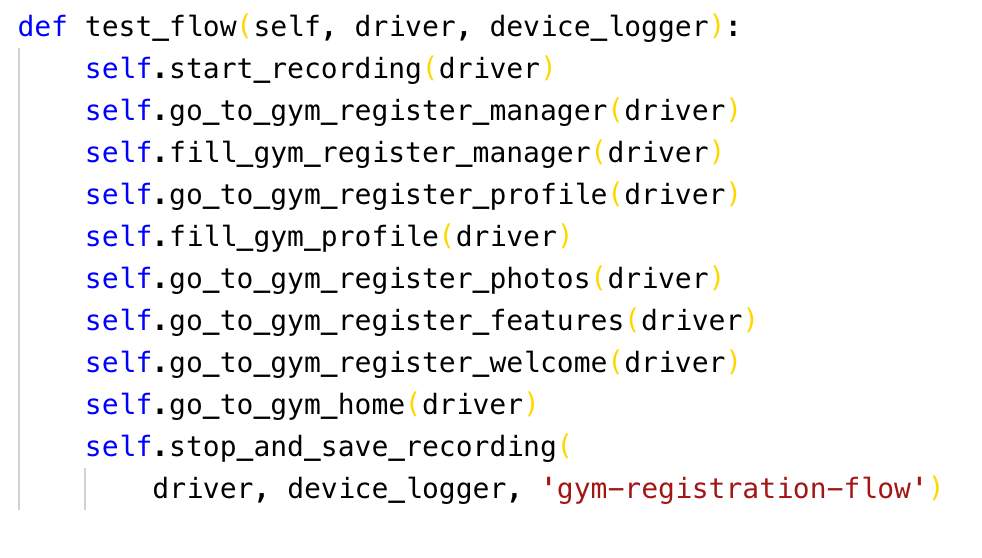
\includegraphics[width=\textwidth]{pfc/figuras/test-flow-appium.png}
        \caption{Appium}
        \label{fig:test-flow-appium}
    \end{subfigure}
    ~
	\begin{subfigure}[b]{0.3\textwidth}
        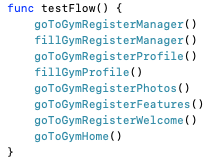
\includegraphics[width=\textwidth]{pfc/figuras/test-flow-earlgrey.png}
        \caption{EarlGrey}
        \label{fig:test-flow-earlgrey}
    \end{subfigure}
    ~
    \caption{Funções de teste do fluxo de cadastro das academias}
    \label{fig:test-flow}
\end{figure}

\begin{figure}[H]
    \centering
    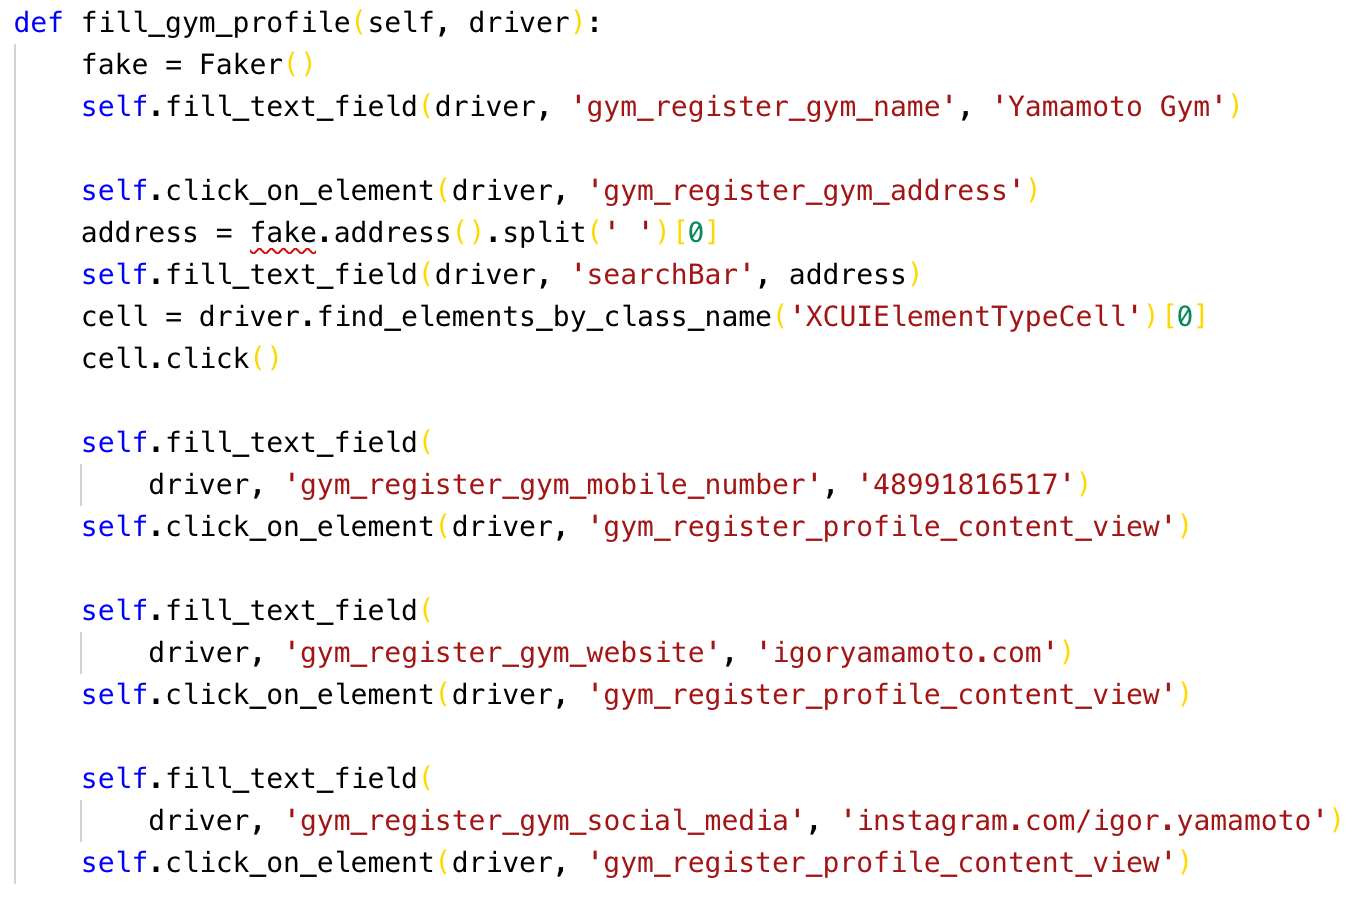
\includegraphics[width=0.8\textwidth]{pfc/figuras/fill-gym-appium.png}
    \caption{Detalhe de implementação de um método do caso de teste que realiza os comandos para interação com a interface gráfica - Appium}
    \label{fig:fill-gym-appium}
\end{figure}

\begin{figure}[H]
    \centering
    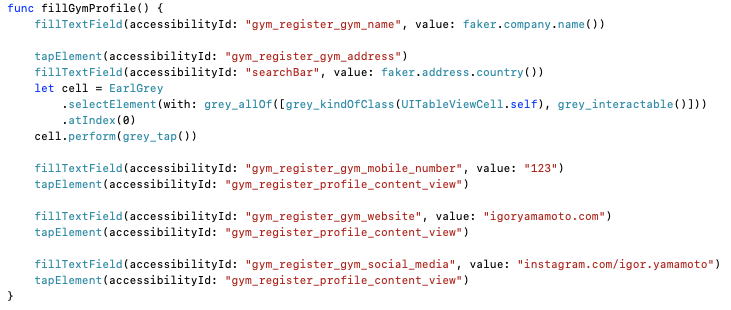
\includegraphics[width=0.8\textwidth]{pfc/figuras/fill-gym-earlgrey.png}
    \caption{Detalhe de implementação de um método do caso de teste que realiza os comandos para interação com a interface gráfica - EarlGrey}
    \label{fig:fill-gym-earlgrey}
\end{figure}

\subsection{Erros de Cadastro do Treinador}
Este caso tem como objetivo testar as mensagens (Figura \ref{fig:error-messages-test}) e estados de erro (Figura \ref{fig:error-states-test}) no preenchimento das informações de usuário do treinador (Figura \ref{fig:register-trainer-info}). O teste tem sucesso se as mensagens correspondem às esperadas para cada caso de erro.

A implementação deste caso foi feita de forma exaustiva, ou seja, todas as combinações possíveis de entradas de campo de texto foram testadas, considerando duas opções para cada entrada: válida ou inválida. Como exemplo, o campo de e-mail teve a entrada "igor@jungledevs.com" considerada válida e a entrada "invalidemail", inválida.

A implementação deste cenário de teste foi realizada somente no Appium. O uso do EarlGrey para este caso foi julgado desnecessário para o estudo, uma vez que o primeiro caso já indicou que a implementação seria semelhante e que informações suficientes para o comparativo entre as ferramentas já haviam sido coletadas. Além disso, a execução do caso de teste mostrou-se demasiadamente lenta, pelo fato de ser exaustiva.

\begin{figure}[H]
	\centering
    \begin{subfigure}[b]{0.3\textwidth}
        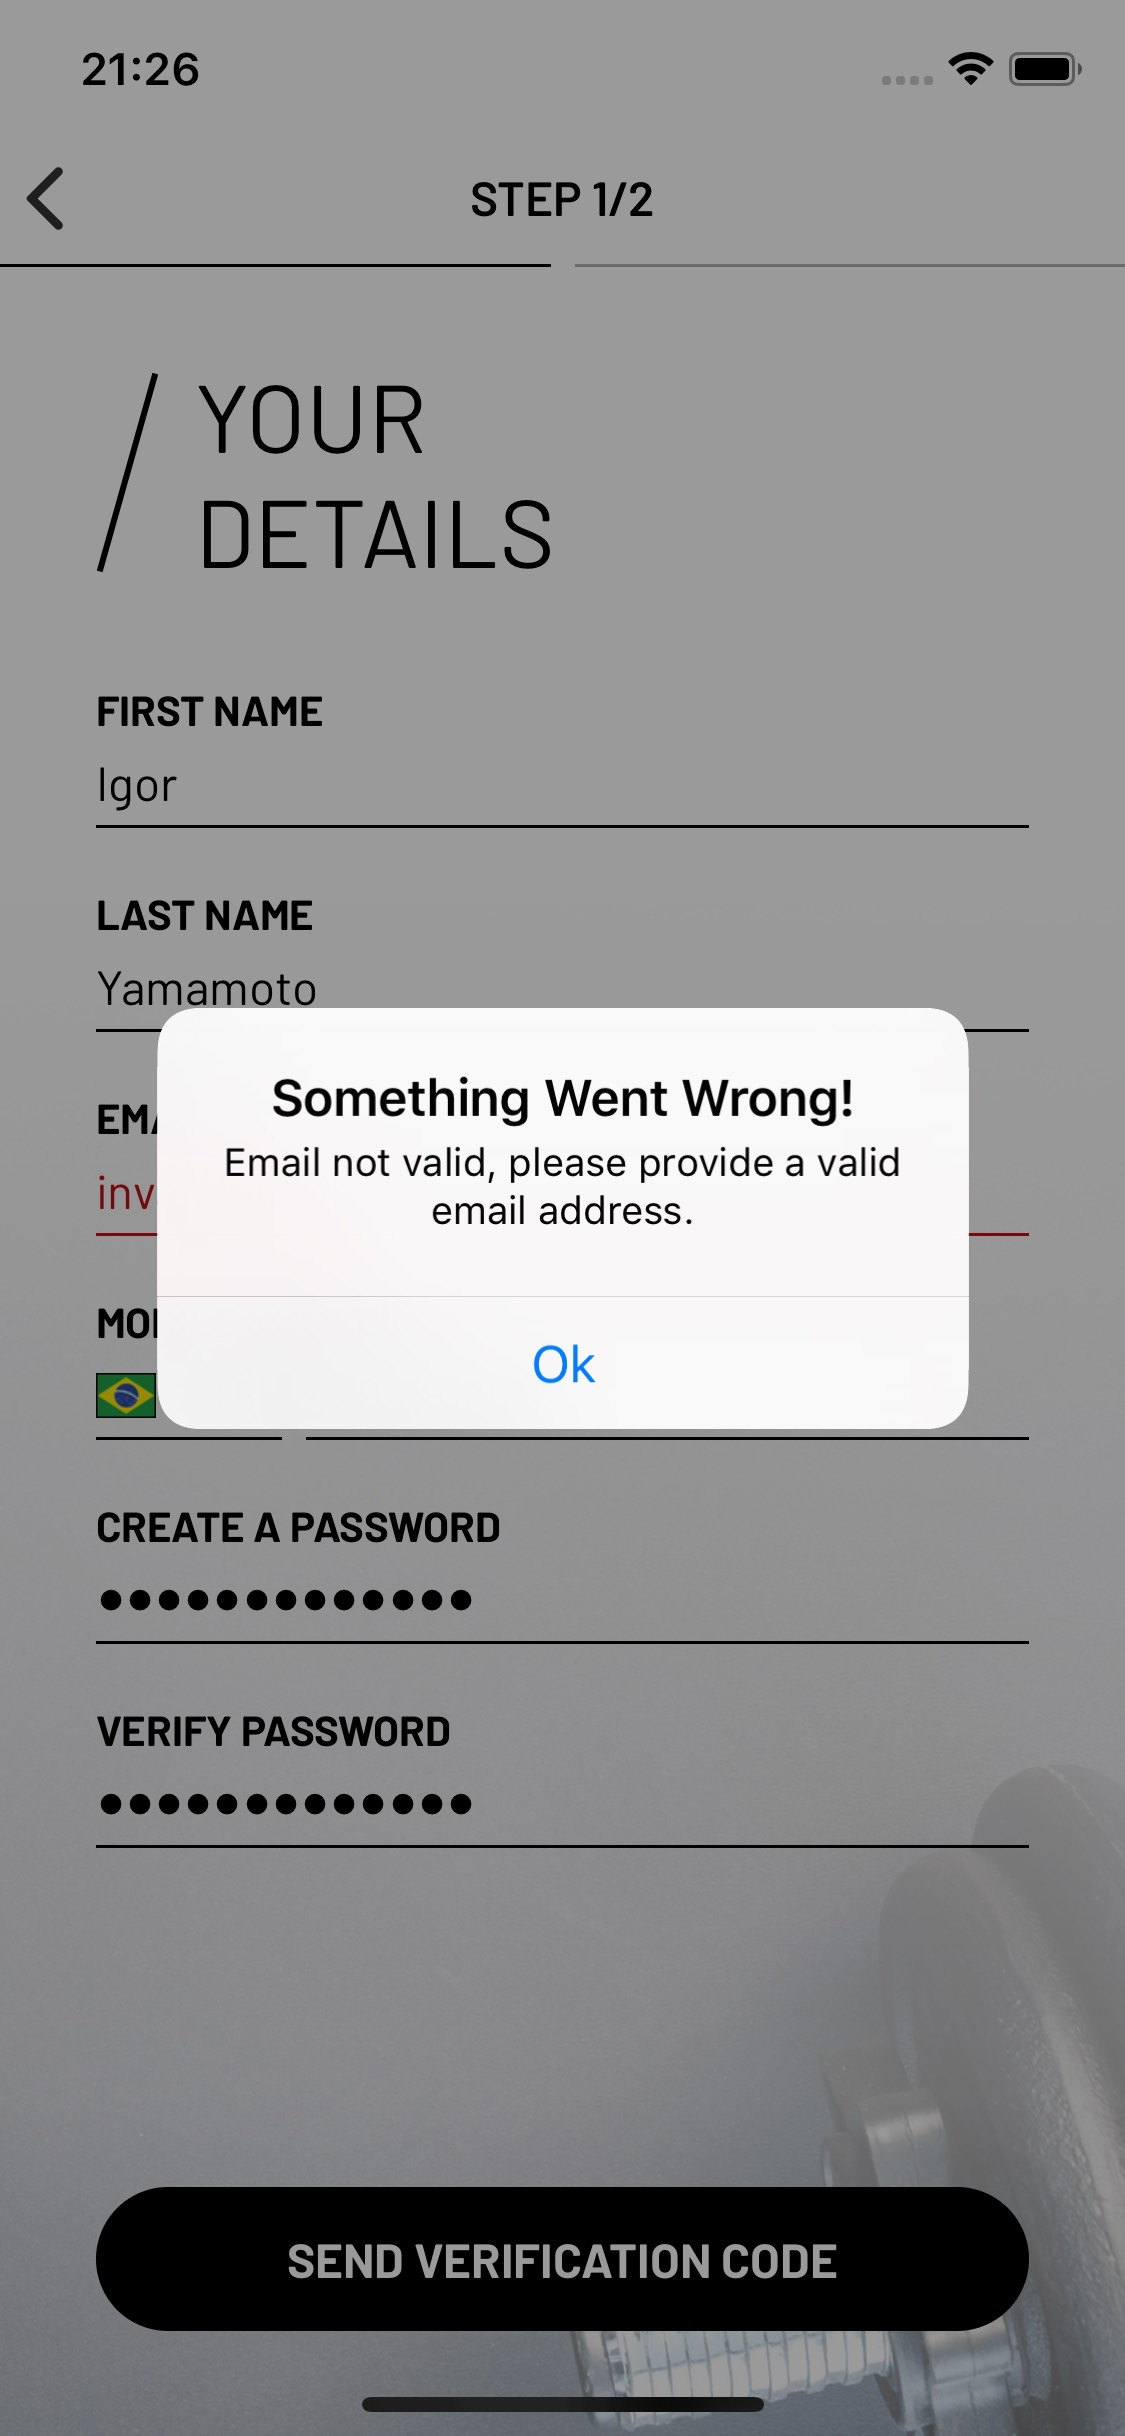
\includegraphics[width=\textwidth]{pfc/figuras/email-not-valid.png}
        \caption{E-mail inválido}
        \label{fig:email-not-valid}
    \end{subfigure}
    ~
	\begin{subfigure}[b]{0.3\textwidth}
        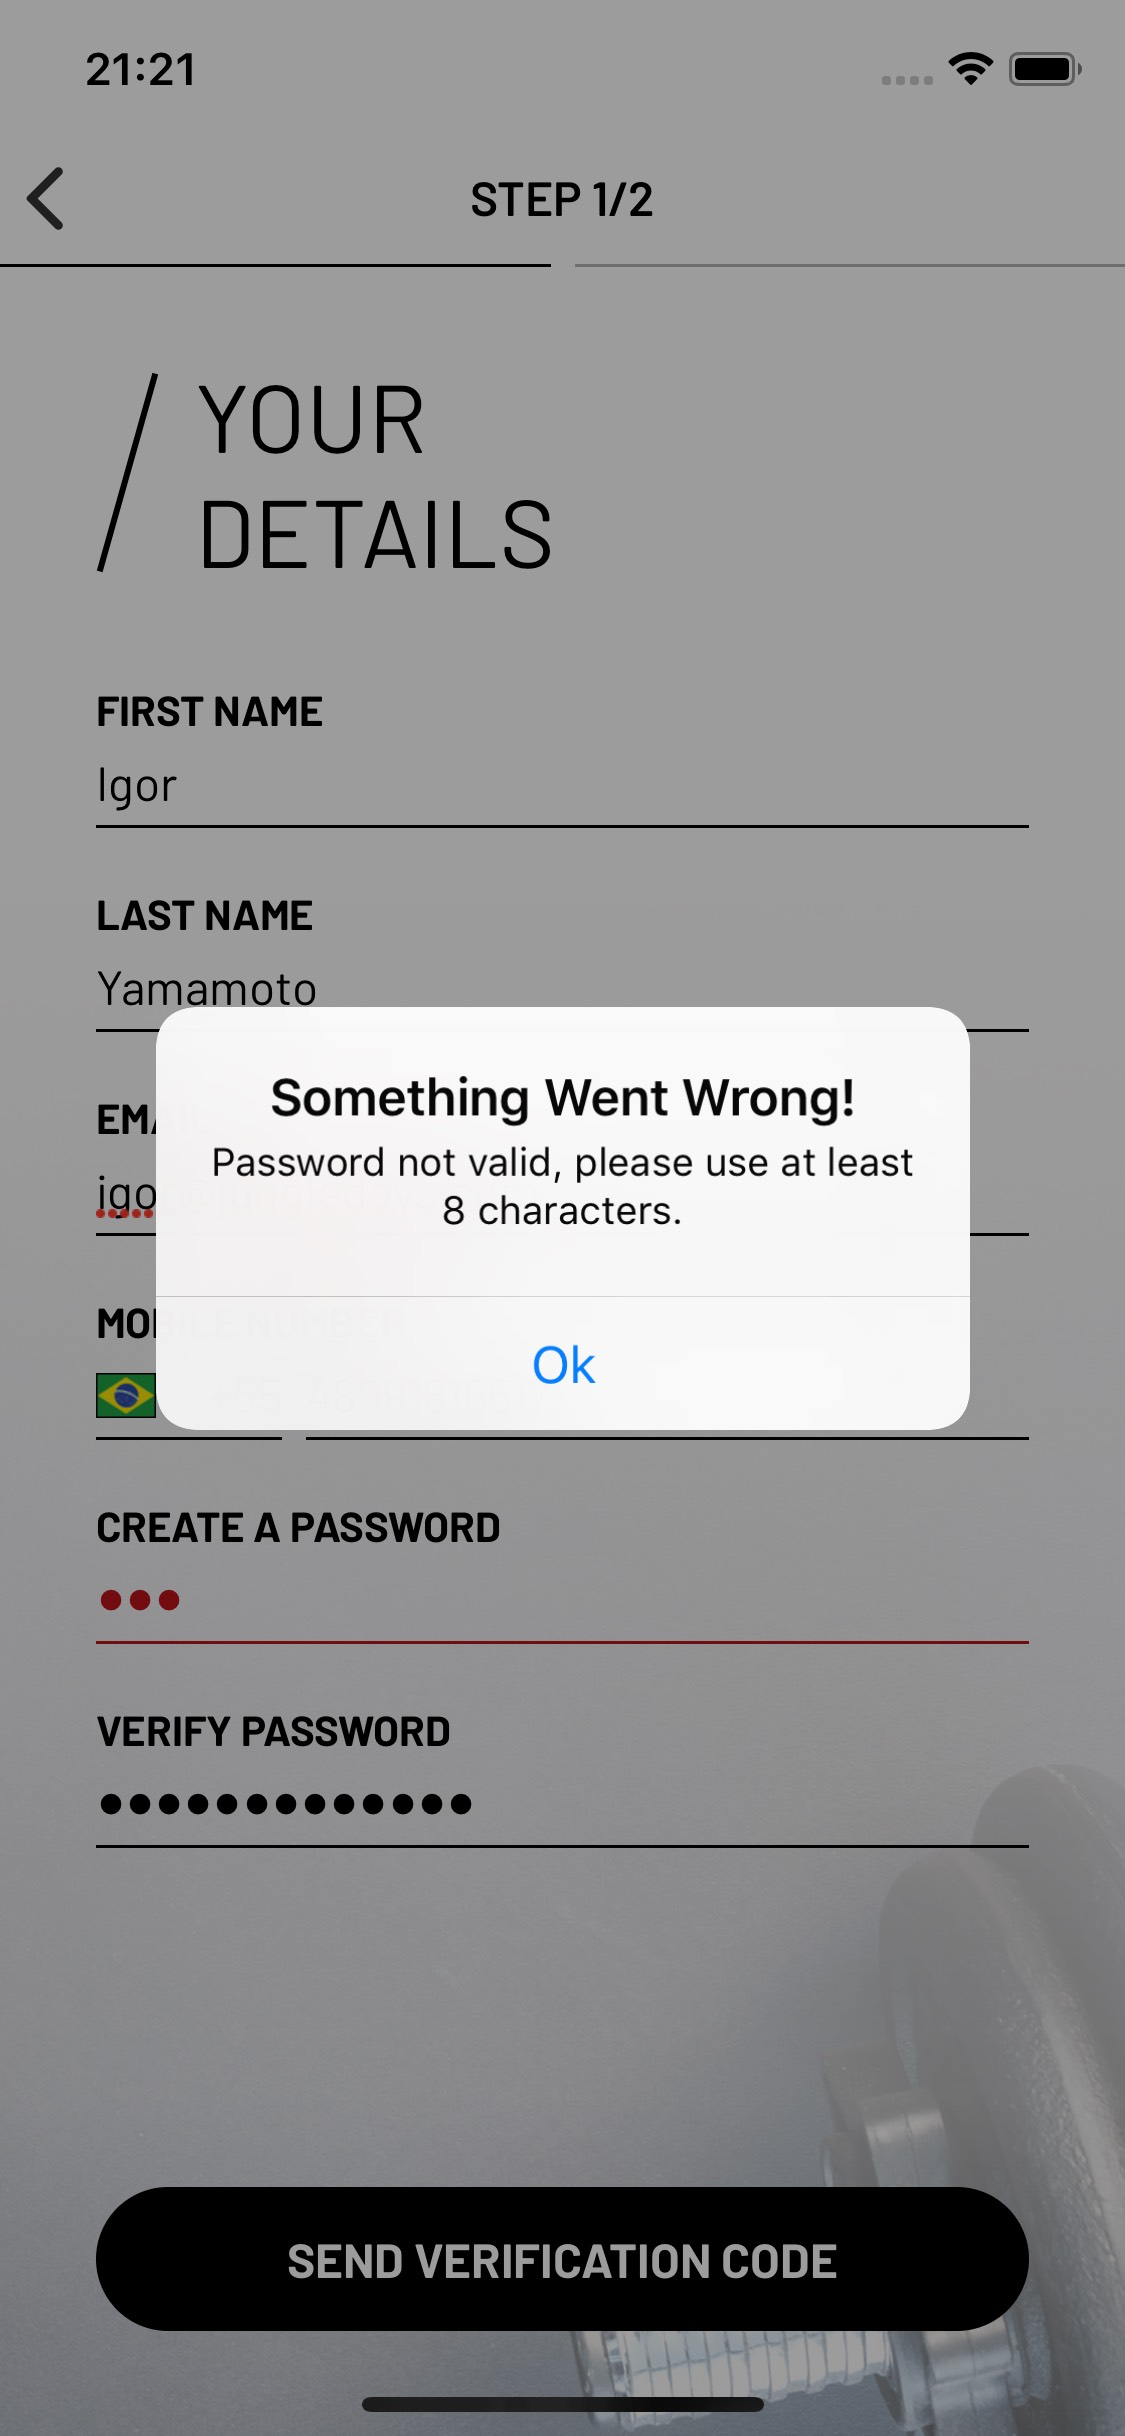
\includegraphics[width=\textwidth]{pfc/figuras/password-not-valid.png}
        \caption{Senha inválida}
        \label{fig:password-not-valid}
    \end{subfigure}
    ~
    \begin{subfigure}[b]{0.3\textwidth}
        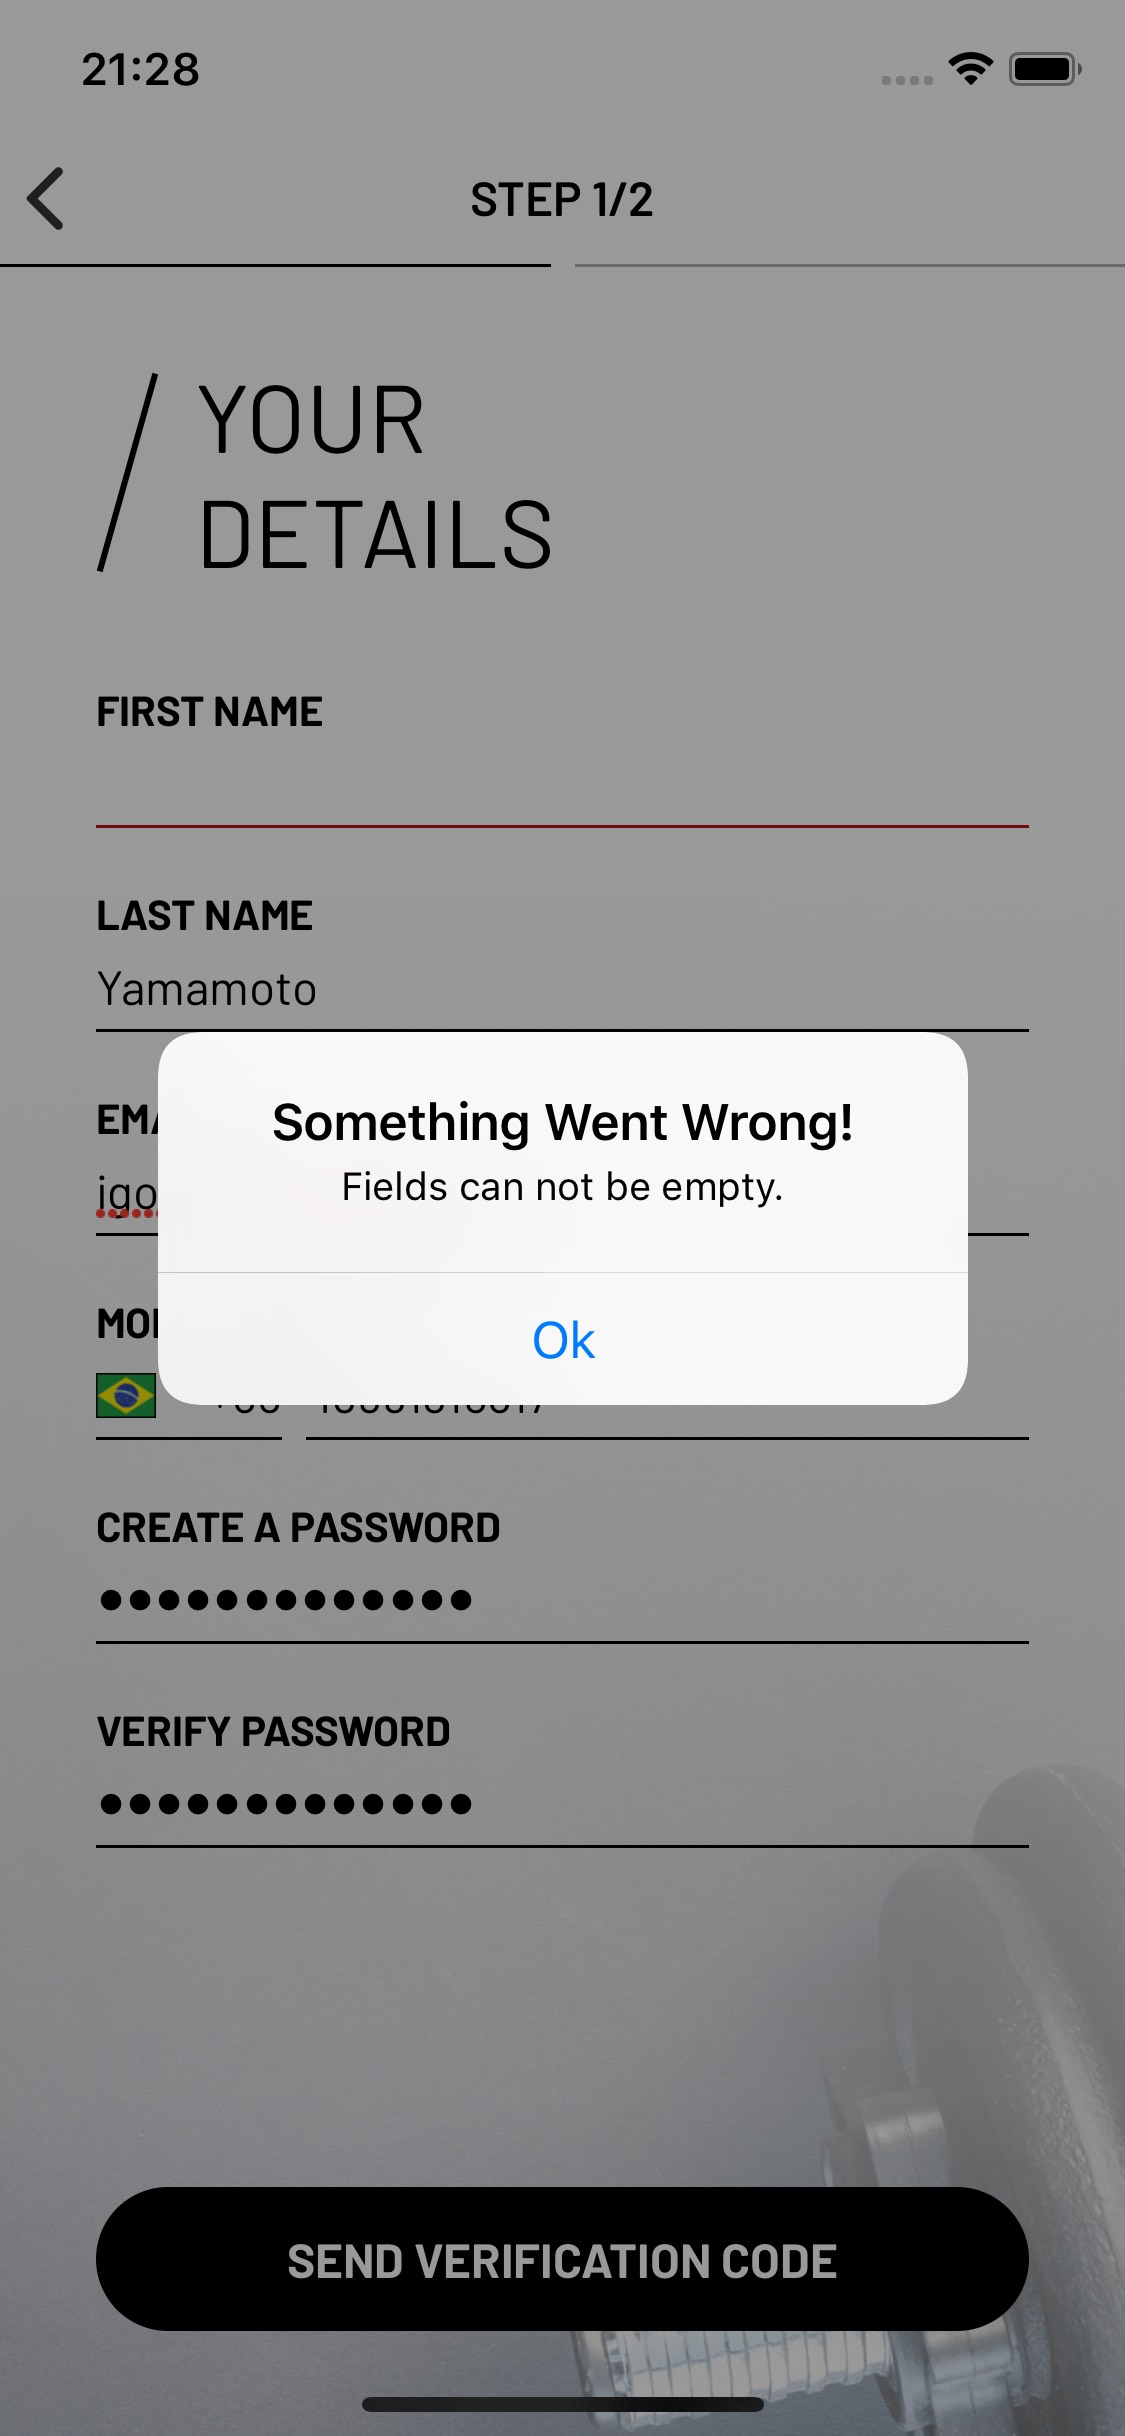
\includegraphics[width=\textwidth]{pfc/figuras/fields-empty.png}
        \caption{Campo nulo}
        \label{fig:empty-fields}
    \end{subfigure}
    ~
    \caption{Mensagens de erro testadas no cadastro de usuário}
    \label{fig:error-messages-test}
\end{figure}

\begin{figure}[H]
	\centering
    \begin{subfigure}[b]{0.4\textwidth}
        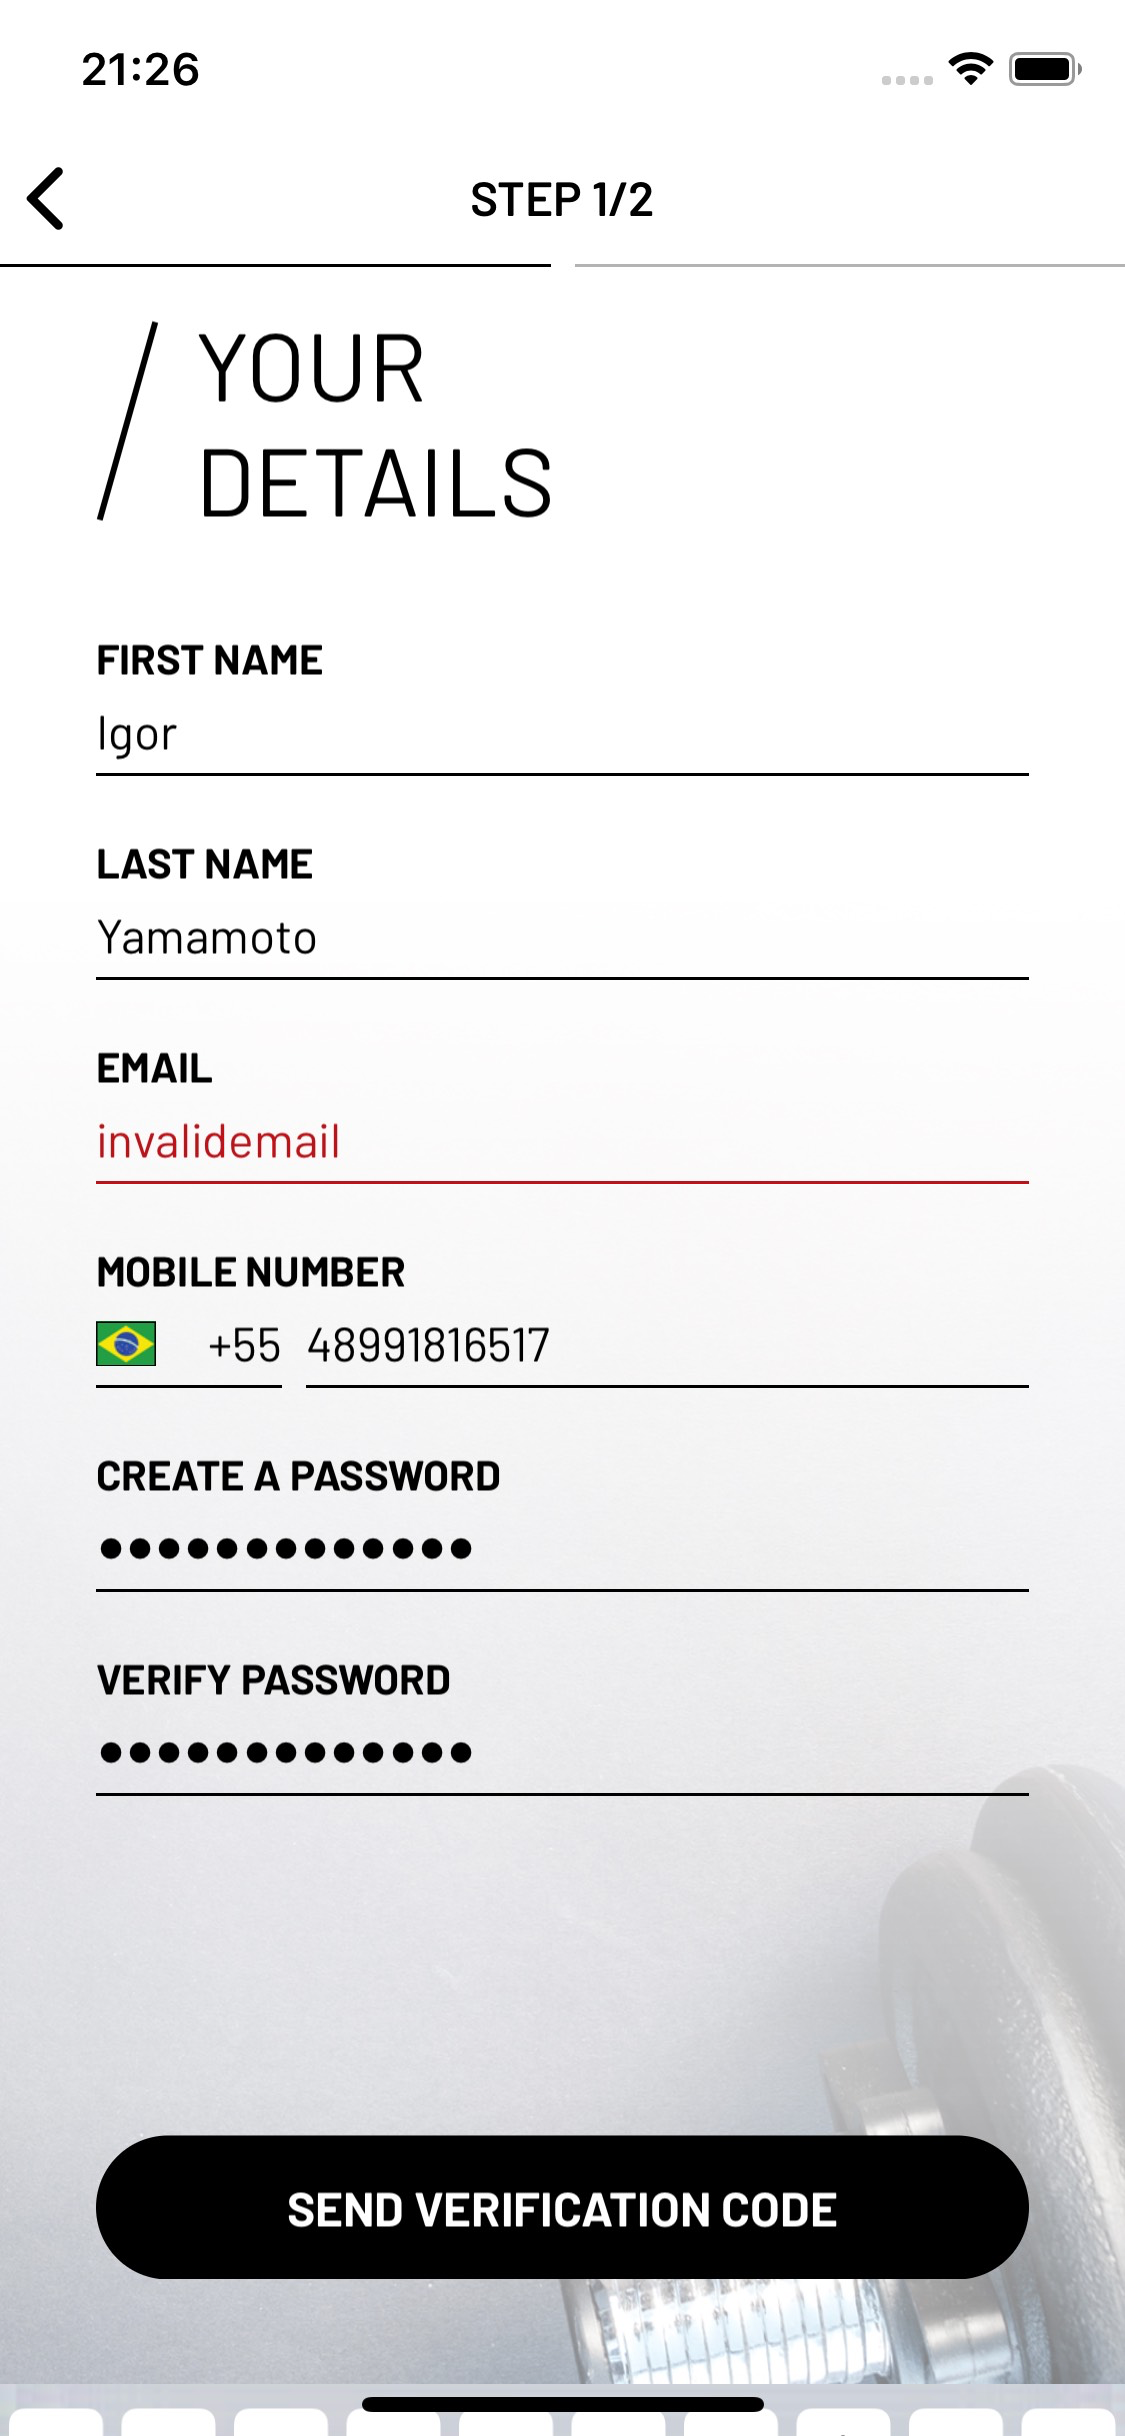
\includegraphics[width=\textwidth]{pfc/figuras/email-not-valid-field.png}
        \caption{Email inválido}
        \label{fig:email-not-valid-field}
    \end{subfigure}
    ~
	\begin{subfigure}[b]{0.4\textwidth}
        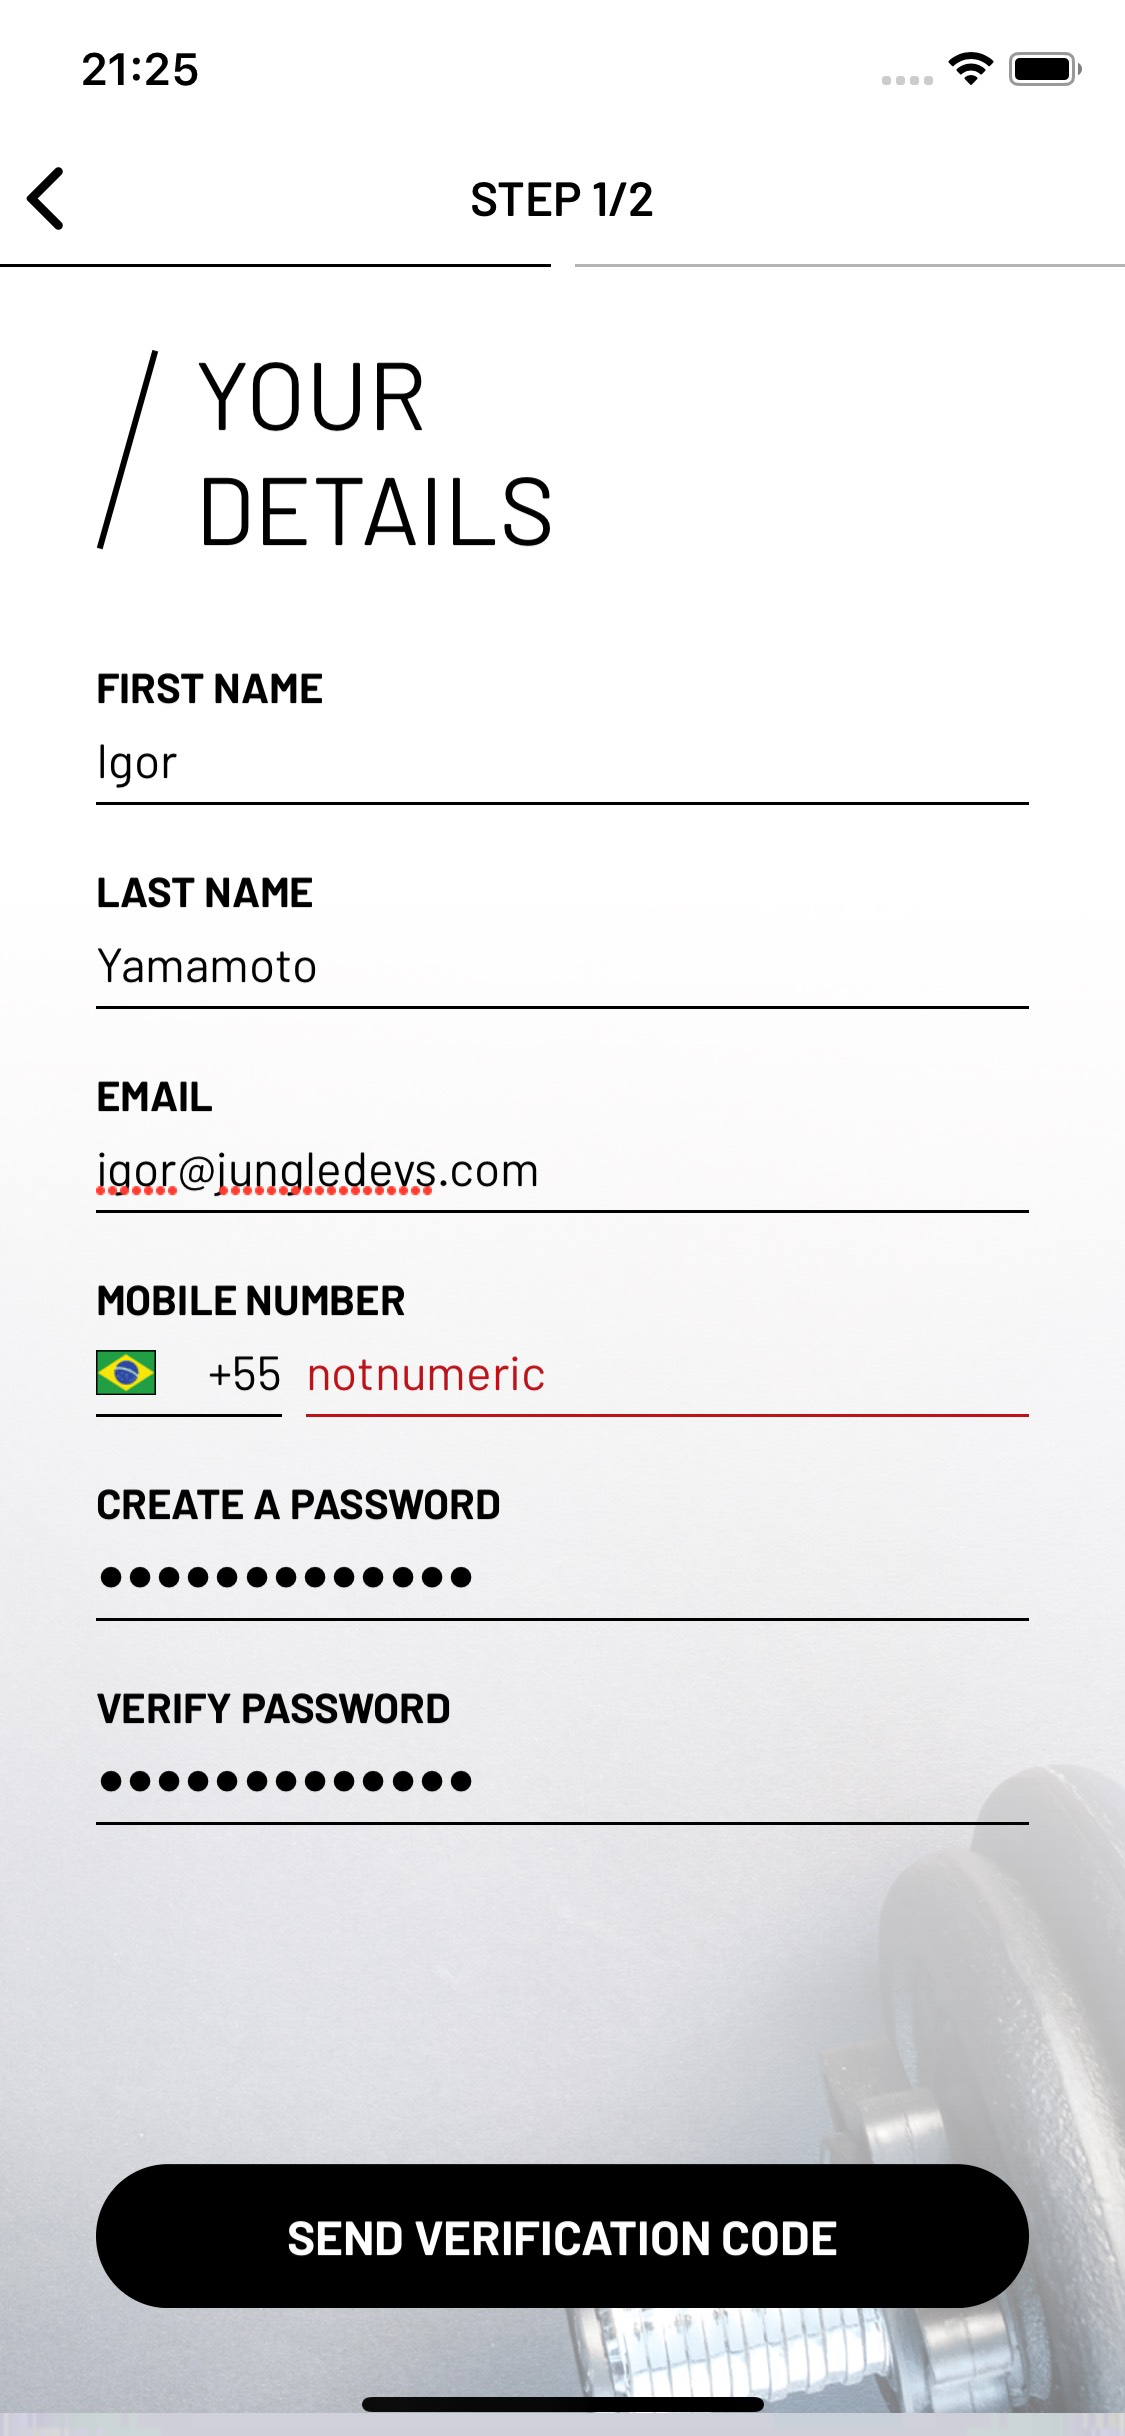
\includegraphics[width=\textwidth]{pfc/figuras/phone-not-valid-field.png}
        \caption{Número telefônico inválido}
        \label{fig:phone-not-valid-field}
    \end{subfigure}
    ~
    \caption{Estados de erro testados no cadastro de usuário}
    \label{fig:error-states-test}
\end{figure}

\section{Dificuldades e Limitações do Estudo}
A maior dificuldade de implementação encontrada foi o setup das ferramentas, em particular do Appium. Esta etapa demandou uma porção de tempo considerável em relação ao total despendido para o estudo. A dificuldade foi decorrente da inexperiência da realização do processo pelos membros da empresa e pelo autor. O Appium exigiu um esforço extra por se tratar de uma ferramenta externa ao ambiente de desenvolvimento iOS. Para configurar a ferramenta, foi necessária a instalação de componentes externos de software (como a CLI e GUI do Appium), a instalação de bibliotecas no Python e configuração de integração entre o simulador de dispositivos do Xcode e o servidor web do Appium.

A segunda dificuldade encontrada na condução do estudo foi a identificação de causas de erro na execução dos testes, particularmente no Appium novamente. As mensagens de erro do Appium são mais verbosas que as mensagens do EarlGrey (ver comparação na Figura \ref{fig:error-test-tools}), o que dificulta a identificação da causa do erro.

\begin{figure}[H]
	\centering
    \begin{subfigure}[b]{0.4\textwidth}
        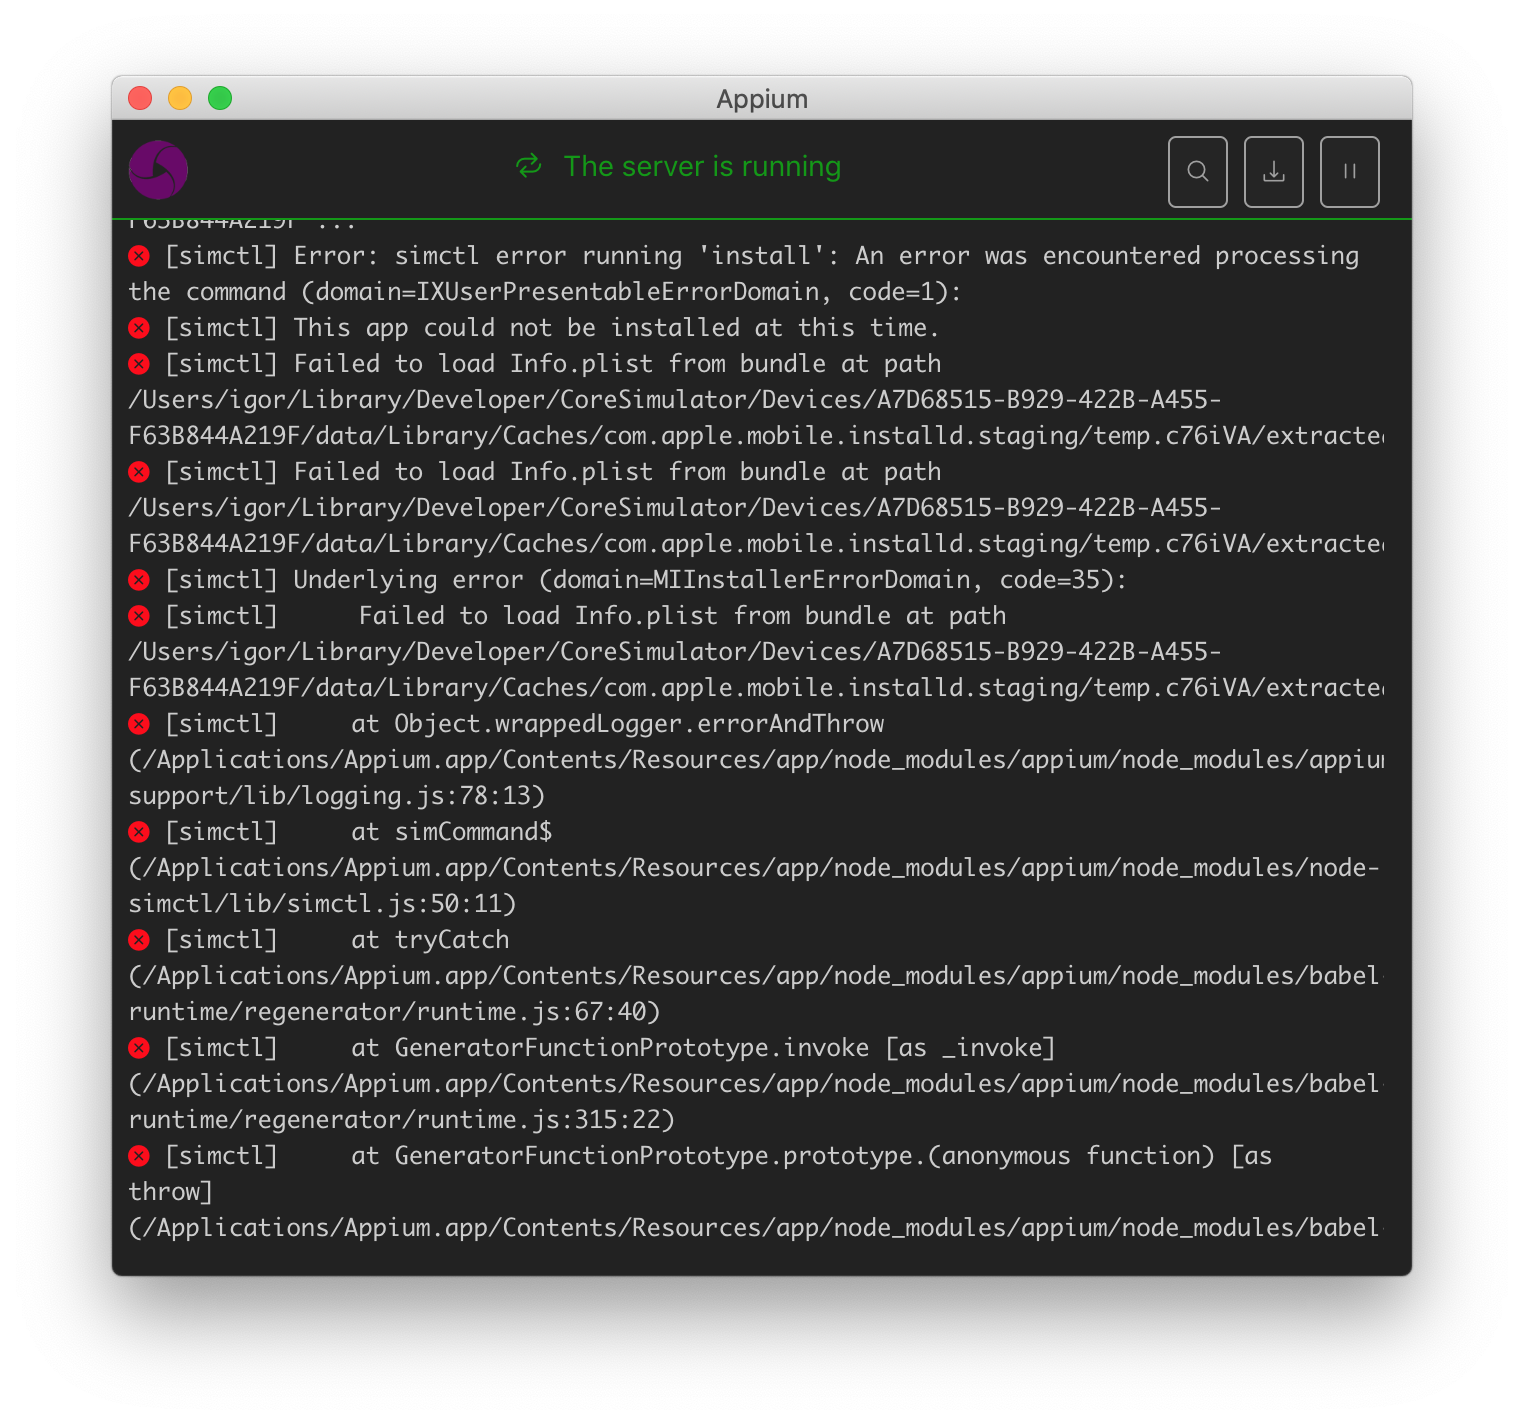
\includegraphics[width=\textwidth]{pfc/figuras/error-appium.png}
        \caption{Erros no Appium}
        \label{fig:error-appium}
    \end{subfigure}
    ~
	\begin{subfigure}[b]{0.4\textwidth}
        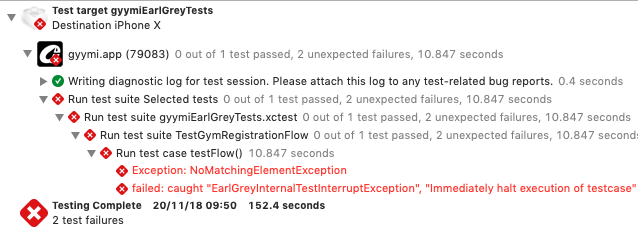
\includegraphics[width=\textwidth]{pfc/figuras/error-earlgrey.png}
        \caption{Erros no EarlGrey}
        \label{fig:error-earlgrey}
    \end{subfigure}
    ~
    \caption{Mensagens de error durante a execução dos testes}
    \label{fig:error-test-tools}
\end{figure}

O estudo esteve limitado a testes no aplicativo iOS, excluindo-se a plataforma Android. O autor não esteve envolvido no desenvolvimento do aplicativo para o sistema Android e, em decorrência deste fator, não foi possível aplicar os testes à plataforma por limitações de tempo. Esta restrição influencia a comparação entre as ferramentas, uma vez que uma dos benefícios do Appium é o suporte à múltiplas plataformas.
